\chapter{マルチスペクトル画像を用いた含水比の推定}
\thispagestyle{empty}
\label{ch:WaterContentEstimation}
\minitoc

%\newcommand{\argmax}{\mathop{\rm arg~max}\limits}
%\newcommand{\argmin}{\mathop{\rm arg~min}\limits}

\newpage

%==============================================================================
%はじめに
%==============================================================================
\section{はじめに}

本章では,非接触での走破性判定のために本研究で提案した,スペクトル画像を用いたコーン指数推定の2つ目のステップである,
スペクトル画像を用いた含水比の推定の詳細について述べる.
本研究の提案手法において,本章で解説する部分を図\ref{fig:thesis_constitution_ch4}に茶色で示す.

% 本研究では,含水比の推定において,スペクトル画像の中でも分光させる波長の数が少ない
% マルチスペクトル画像を使用する.

まず,\ref{sec:EstimationFromSpectrum}節において,
% 水は近赤外の光を吸収し,
同じ種類の土であっても含水比が異なると
分光反射率スペクトルが変動することを利用して,
スペクトル画像から含水比を推定することを述べる.
水は近赤外の光を吸収するため,土に含まれる水の量の指標である含水比が変動すると土の分光反射率も特に近赤外の波長において
減少する.
そこで,これを利用することによって,スペクトル画像から含水比を推定する.% "用いて"の後は"から~"
また,含水比の詳細についても解説する.
% 含水比の解説と,分光反射率スペクトルから含水比を推定する手法の原理について述べる.

次に,\ref{sec:AnalysisOfMultispectralImage}節において,
スペクトル画像を用いた含水比推定の詳細を述べる.
水は近赤外の広い範囲の波長の光を吸収するため,
1つの波長帯あたりの幅を広く取ることができるマルチスペクトル画像を使用する.
従って,マルチスペクトル画像から水が光を吸収する近赤外の波長帯と水が光を吸収しない波長帯の分光反射率を取得し,
その2つの分光反射率を用いて含水比を推定する.

最後に,\ref{sec:PreliminaryExperimentOfEstimation}節において,
\ref{sec:AnalysisOfMultispectralImage}節で述べた手法の
有効性を確認するために実施した,マルチスペクトル画像を用いた含水比推定の検証実験の詳細について述べる.% "詳細"がつく場合と付かない場合では詳しさが明確に異なる.

\begin{figure}[p]
	\begin{center}
	\centering
	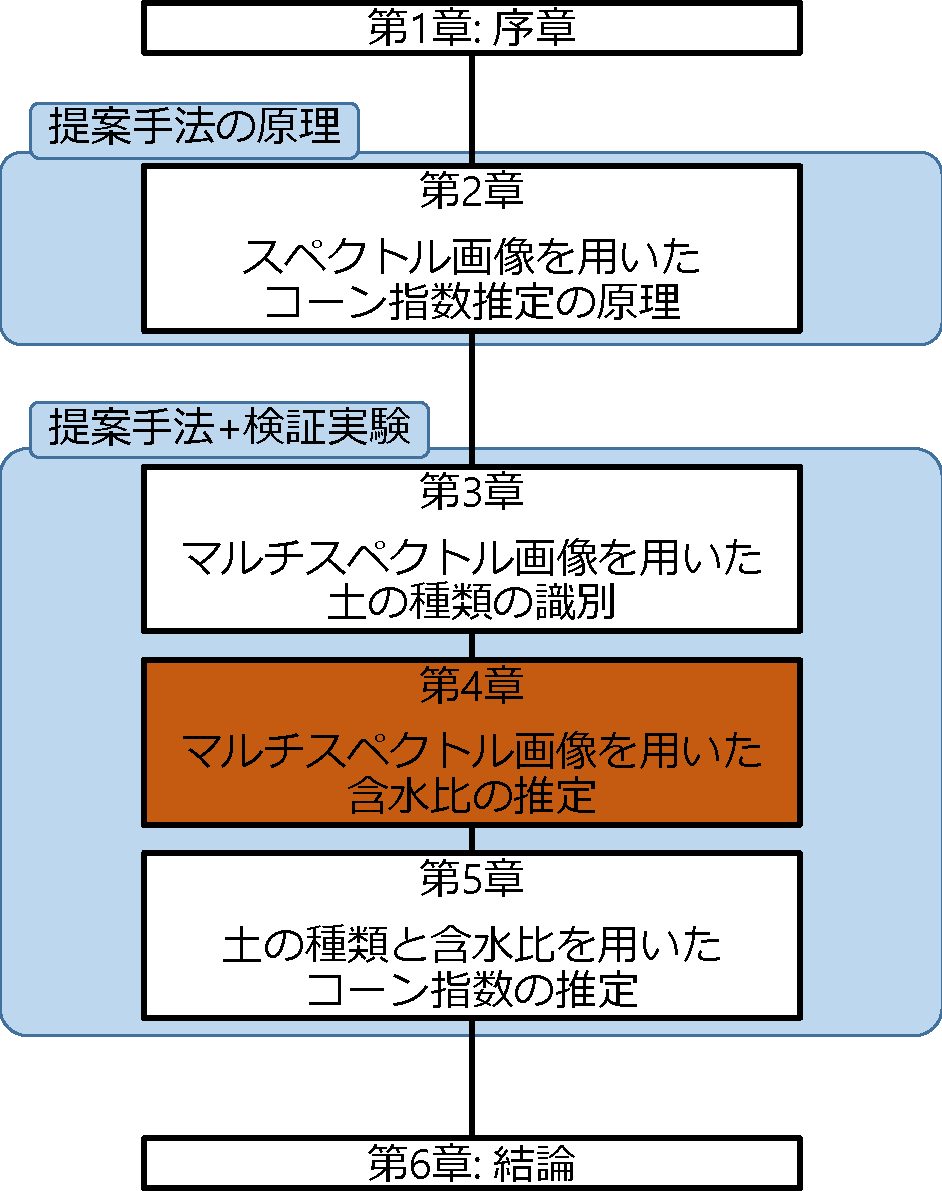
\includegraphics[width=8cm]{./Ch4_WaterContentEstimation/Fig/thesis_constitution_ch4_compressed.pdf}
	\caption{本章で解説する部分(茶色の部分)}\label{fig:thesis_constitution_ch4}
	\end{center}
\end{figure}

\clearpage

%==============================================================================
%分光反射率スペクトルを用いた含水比の推定
%==============================================================================
\section{分光反射率スペクトルを用いた含水比の推定}
\label{sec:EstimationFromSpectrum}

\subsection{含水比}
\label{ssec:WaterContent}

含水比は,土に含まれる水の量を示す土質パラメータであり,
土に含まれる土の粒子の質量に対する,同じ土に含まれる水の質量の比を示す土質パラメータである.
含水比を算出する式を\mbox{式(\ref{eq:watercontent_measurement})}に示す\cite{日本建設総合試験所2019}.

\begin{eqnarray}
含水比 = \frac{m_w}{m_s}, \label{eq:watercontent_measurement}
\end{eqnarray}

\mbox{式(\ref{eq:watercontent_measurement})}において,$m_w$,$m_s$は,それぞれ土に含まれる水の質量と土粒子の質量を示す.
$m_s$は,採取した土を乾燥炉に入れて水分を蒸発させることで測定する.
また,$m_w$は,採取した直後の土と乾燥させた後の土の質量の差から求められる.

土に含まれる空気,水,土粒子の関係を,図\ref{fig:watercontent_measurement}に示す.
土は,図\ref{fig:watercontent_measurement}に示すように,固体である土粒子,そして土粒子の間
に入り込んだ水と空気から出来ている.
\ref{ssec:ConeindexEstimation}項で述べた通り,土の粒子と水の質量の比である含水比が,コーン指数に大きく影響する.

\begin{figure}[bp]
      \begin{center}
            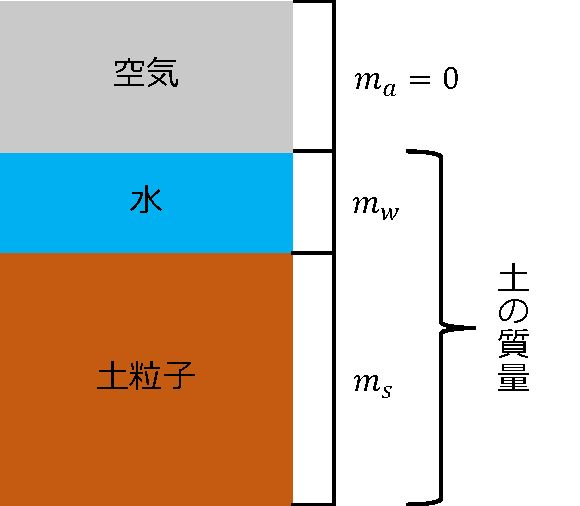
\includegraphics[width=7cm]{./Ch4_WaterContentEstimation/Fig/watercontent_measurement_compressed.pdf}
            \vspace{1cm}
            \caption{土に含まれる空気,水,土粒子の関係(\cite{日本建設総合試験所2019}を参考に作成)}
            \label{fig:watercontent_measurement}
      \end{center}
\end{figure}

\clearpage

\subsection{含水比と分光反射率スペクトルの関係}
\label{ssec:RelationshipBetweenSpectrumAndWaterContent}

% \ref{ssec:ConeindexEstimation}節で述べた通り,コーン指数は土の種類と含水比に大きな影響を受ける.
% そこで,コーン指数を非接触で推定するためには,土の種類の識別と含水比を非接触で推定する.

\ref{ssec:Spectrum}項で述べた通り,分光反射率スペクトルを用いた物質の種類の識別や状態の推定が可能である.
従って,含水比が変化した場合も,その土の分光反射率スペクトルが変動する.
水分子は,それを構成する酸素原子と水素原子の間の振動収縮と変角運動によって
特に近赤外の光を吸収することが知られている\cite{李2000}\cite{Lobell2002}\cite{Tian2015}.% 引用

含水比の違いによって,土の分光反射率スペクトルが異なるグラフを図\ref{fig:watercontent_and_spectrum_relationship}に示す.
この図において,縦軸が分光反射率,横軸が波長を示しており,描かれている3本の黒い曲線が土の分光反射率スペクトルを
示している.
この3本は同じ土の種類の分光反射率スペクトルであるが,上にある曲線から下にある曲線に行くに従って
含水比が高くなっており,上の曲線から順に,含水比が低い,真ん中,高い順に並んでいる.
そして,水が光を吸収しない波長帯が茶色で示され,水が光を吸収する波長帯である近赤外の波長帯が水色で示されている.
含水比が増えると土粒子の隙間に水が入り込み,空気と土の間の屈折率の差が減少するため,
空気中から土への入射光の内,反射せずに土の中に屈折して進入していく光の割合が増える.
従って,含水比の増加に伴って分光反射率スペクトルは全体的に低くなる.
しかし,その作用とは別に,水は水分子の酸素原子と水素原子の間の振動収縮と変角運動のために
近赤外の光を吸収するため,分光反射率スペクトル全体のなかでも,特に近赤外の % "波長"という単語はグラフの軸の説明にのみ使用
分光反射率が大きく減少する.
この性質を利用することで分光反射率スペクトルから含水比を推定する.
具体的には,図\ref{fig:watercontent_and_spectrum_relationship}のグラフにおいて,含水比が1番低い状態における2つの波長帯の分光反射率の差を$d_1$,
含水比が真ん中の状態における差を$d_2$,
含水比が1番高い状態における差を$d_3$とすると,
\begin{eqnarray}
d_1 > d_2 > d_3, \label{eq:spectrumDiff}
\end{eqnarray}
となっていることが分かる.
この\mbox{式(\ref{eq:spectrumDiff})}より,含水比が増加すると,
水が光を吸収する近赤外の波長帯の分光反射率から水が光を吸収しない波長帯の分光反射率を
引いた差は逆に減少することが分かる.
これを利用して含水比を推定する.

\begin{figure}[b]
      \begin{center}
            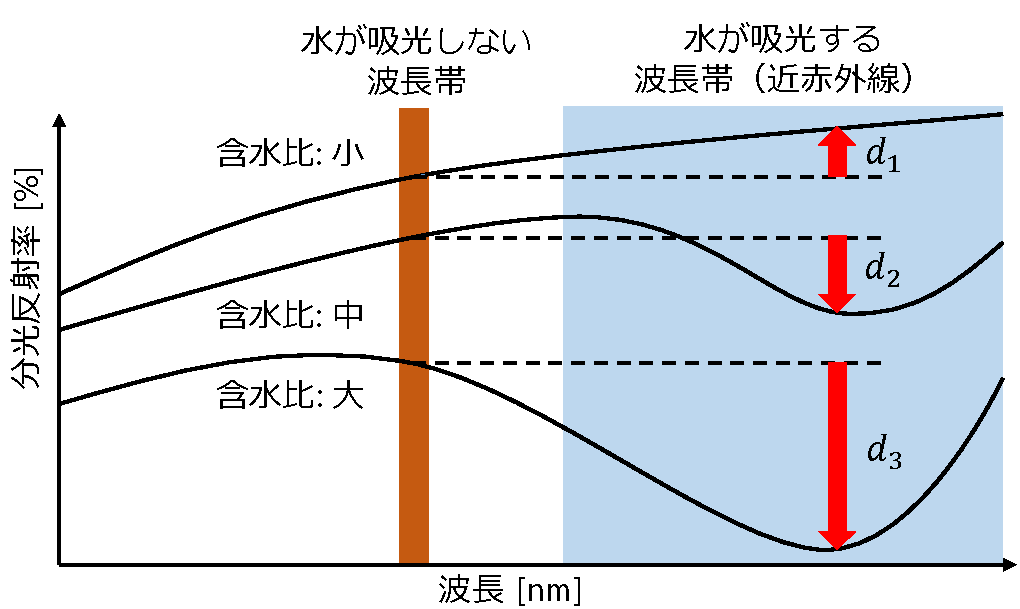
\includegraphics[width=12cm]{./Ch4_WaterContentEstimation/Fig/watercontent_and_spectrum_relationship_compressed.pdf}
            \caption{同一種類の土における含水比の増加に伴う分光反射率の減少}
            \label{fig:watercontent_and_spectrum_relationship}
            \vspace{3cm}
      \end{center}
\end{figure}



水分子が近赤外の光を吸収する原因となる酸素原子と水素原子の間の振動収縮と変角運動は,
水分子の周囲に存在する他の水分子との水素結合の数と方向に大きく左右される\cite{中島2015}.
そしてその水素結合の数と方向は温度や湿度に大きく影響される\cite{角田2013}.
従って,水は,温度や湿度によって最も光を吸収する波長帯を変化させるため,
近赤外において広い範囲の光を吸収する.

% ここにもう1つ項(土の種類の識別に必要な分光反射率スペクトルの要件)を入れて,波長分解能についてより詳しく述べる
% なぜマルチスペクトル画像を使用する必要があるのか?

従って,近赤外の光の分光反射率を用いて含水比を推定するためには,
近赤外の幅広い範囲の光を取得するスペクトル画像を用いる必要がある.
そのため,本研究では,スペクトル画像のなかでも,入射光を分光させる波長帯の数が少なく,
近赤外の幅広い範囲の光を取得することが
できるマルチスペクトル画像を用いる.

\clearpage

%==============================================================================
%マルチスペクトル画像の解析
%==============================================================================
\section{マルチスペクトル画像の解析}
\label{sec:AnalysisOfMultispectralImage}

\subsection{波長帯の数が少ないマルチスペクトル画像}
\label{ssec:MultispectralImage}

マルチスペクトル画像とは,\ref{sec:HyperAndMultiImages}で述べた通り,一般的なRGB画像が取得するR,G,Bの3波長帯以外の波長帯も取得するスペクトル画像である.
% 一般的には,分光させた波長帯の数は4以上9以下であると言われている.% マルチスペクトル画像の波長数が4~9であることはここで終わり
取得する波長帯の数が少ないマルチスペクトル画像は,スペクトル画像が使われ出した当初から使用されており,
顔の色素の分布や建材の塗装量の調査,工業製品の外観検査に使用されている\cite{中野1996}\cite{長田2004}\cite{田代2013}.% 引用

マルチスペクトル画像の中でも,
取得する波長帯の数が少ないマルチスペクトル画像は,一般的に異なる光学フィルタを装着した,
% 複数のカメラ
並列に並んだ複数の撮像素子
を用いて各波長帯の光の強さを記録する.
従って,同じ位置にある画素であっても,波長帯が異なると映している場所が異なる.
そこで,\ref{ch:SoilTypeDiscrimination}章で使用した,取得する波長帯の数が非常に多いスペクトル画像の場合とは違って,画素ごとに分光反射率スペクトルを取得するのではなく,
まず水が光を吸収する近赤外の波長帯とそれ以外の水が光を吸収しない波長帯の,2つの波長帯を取得した
後,それぞれの波長帯で同じ場所を映している画素を選んで分光反射率を計算する.
最後に,その差を用いて含水比を推定する.
% \begin{figure}[p]
% 	\begin{center}
% 	\centering
% 	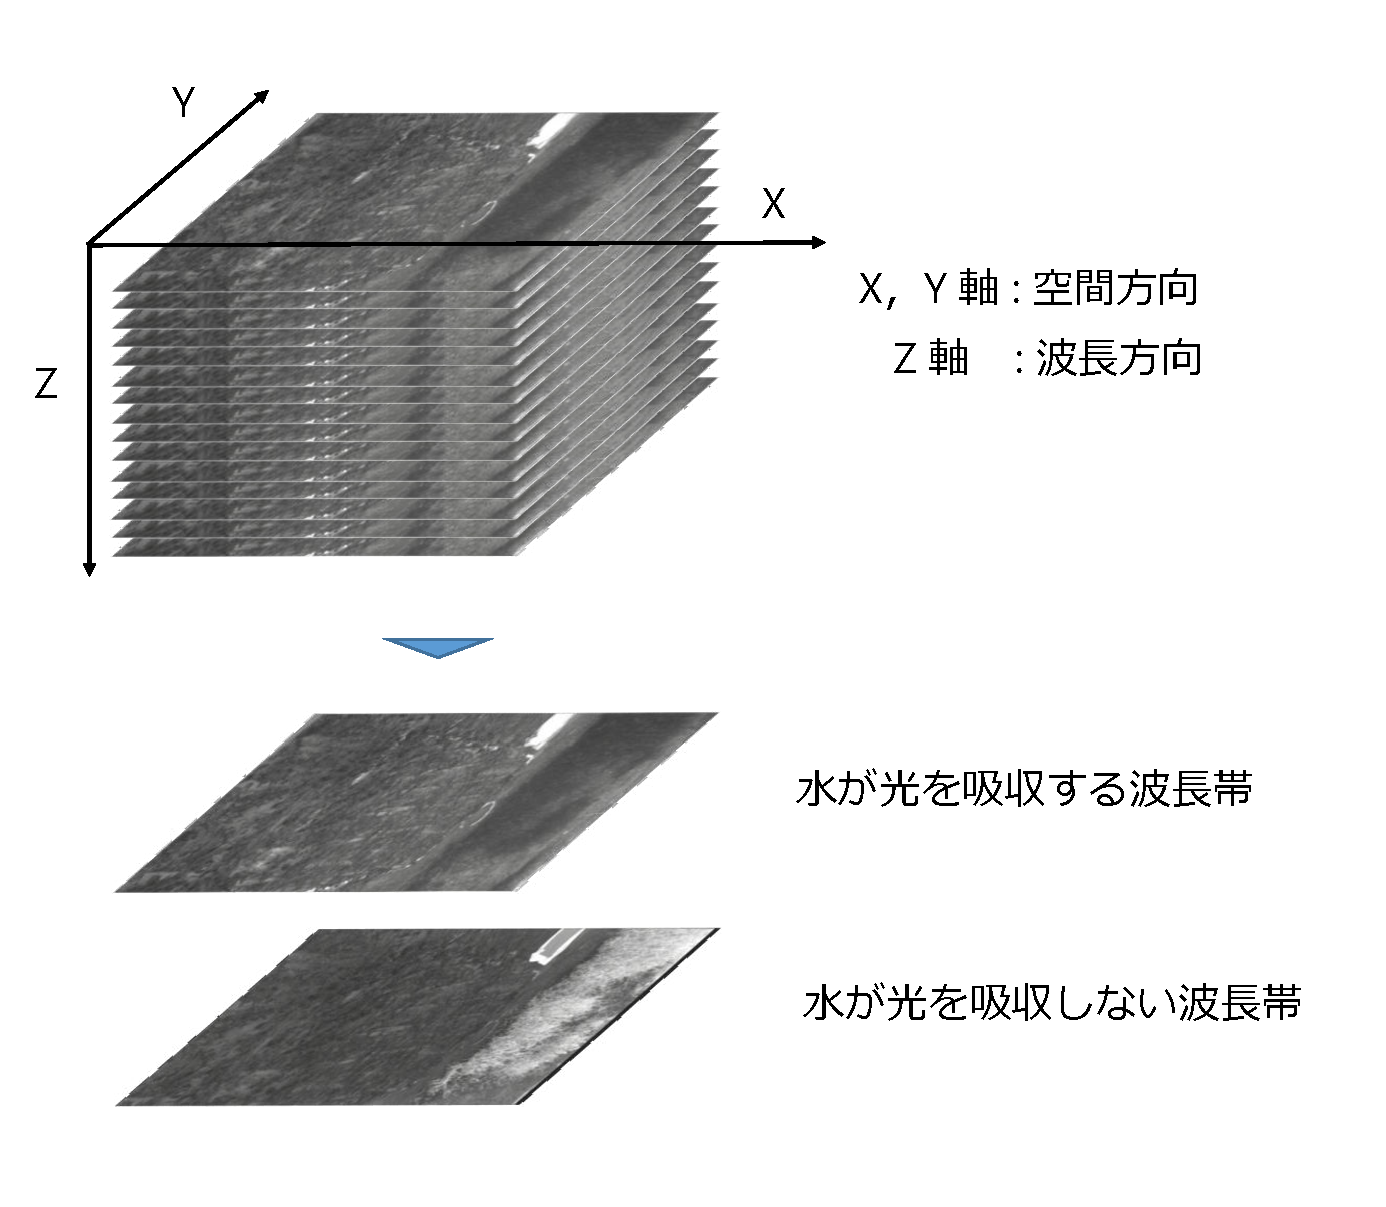
\includegraphics[width=12cm]{./Ch4_WaterContentEstimation/Fig/spectral_image_extraction_compressed.pdf}
% 	\caption{マルチスペクトル画像からの2つの波長帯の抽出}\label{fig:spectral_image_extraction}
% 	\end{center}
% \end{figure}

\clearpage

\subsection{分光反射率の解析}
\label{ssec:AnalysisOfSpectrum}

本研究では,水が光を吸収する近赤外の波長帯として900 $\sim$ 1700nmの波長帯を,水が光を吸収しない波長帯として570nmの波長帯を使用する.
同じ種類の土で含水比が異なるサンプルを作り,屋外において,
それぞれのサンプルを太陽光を光源として撮影したマルチスペクトル画像から取得した900 $\sim$ 1700nmの波長帯と570nmの波長帯
の分光反射率をプロットしたグラフを,図\ref{fig:watercontent_and_spectrum_graph}に示す.
図\ref{fig:watercontent_and_spectrum_graph}のグラフにおいて,縦軸が含水比,横軸が分光反射率を示す.
また,図\ref{fig:watercontent_and_spectrum_graph}のグラフに示されている赤いひし形が,同一種類の土で含水比の異なるサンプルを撮影した各マルチスペクトル画像の570nmの波長帯で計算した分光反射率を
プロットしており,黒いひし形が,同一種類の土で含水比の異なるサンプルを撮影した各マルチスペクトル画像の900 $\sim$ 1700nmの波長帯で計算した分光反射率を示す.
さらに,上記で解説した2つの波長帯の分光反射率の間にある赤い矢印が,2つの波長帯の分光反射率の差$d$を示す.

次に,その2つの波長帯の分光反射率の差と含水比を比較したグラフを,図\ref{fig:watercontent_and_spectrumDiff_graph}に示す.
図\ref{fig:watercontent_and_spectrumDiff_graph}のグラフにおいて,縦軸は先ほどと同じ含水比を示すが,横軸は2つの波長帯の分光反射率の差$d$を示す.
なお,横軸は2つの波長帯の分光反射率の単なる差を示すので,単位は図\ref{fig:watercontent_and_spectrum_graph}のグラフの横軸と同じく$\%$となる.
また,図\ref{fig:watercontent_and_spectrumDiff_graph}のグラフに示されている黒い点は,
各含水比に対する,図\ref{fig:watercontent_and_spectrum_graph}のグラフで示された570nmの波長帯の分光反射率と900 $\sim$ 1700nmの波長帯の分光反射率の差を示す.
この図\ref{fig:watercontent_and_spectrumDiff_graph}のグラフより,含水比が減少するに伴って,2つの波長帯の分光反射率の差$d$が増加していることが分かる.
そこで,このグラフに近似線をフィッティングし,そのフィッティングされた近似線を用いることによって,
マルチスペクトル画像から
含水比を推定する.

\begin{figure}[p]
	\begin{center}
		\begin{tabular}{c}

			\begin{minipage}[t]{\linewidth}
			\hspace{1.5cm}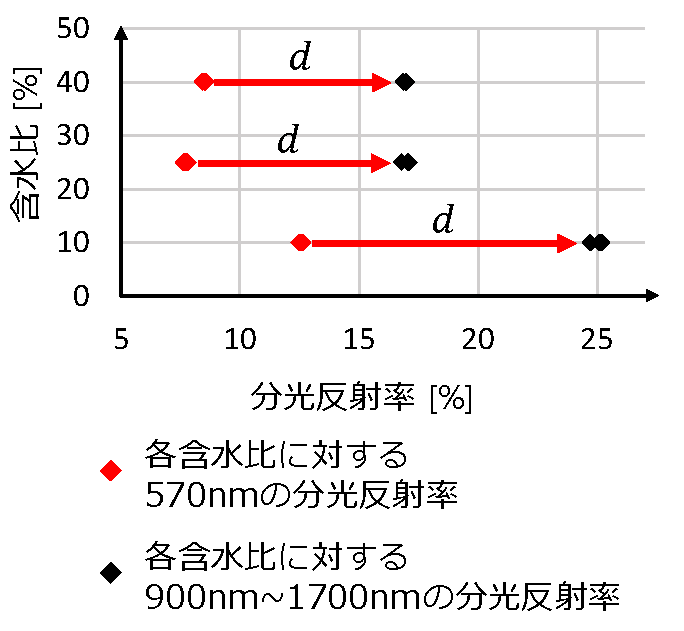
\includegraphics[width=8cm]{./Ch4_WaterContentEstimation/Fig/watercontent_and_spectrum_graph_compressed.pdf}
			\caption{含水比と2つの波長帯の分光反射率の関係}\label{fig:watercontent_and_spectrum_graph}
			\vspace{2cm}
			\end{minipage}

			\\

			\begin{minipage}[b]{\linewidth}
			\hspace{1.5cm}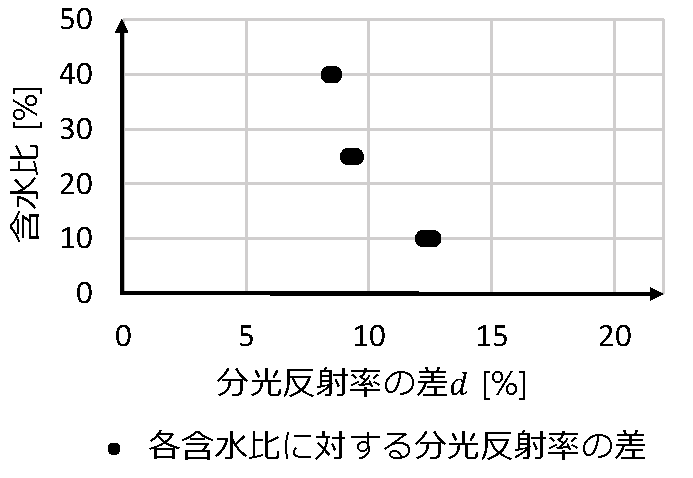
\includegraphics[width=8cm]{./Ch4_WaterContentEstimation/Fig/watercontent_and_spectrumDiff_graph_compressed.pdf}
			\caption{含水比と分光反射率の差の関係}\label{fig:watercontent_and_spectrumDiff_graph}
			\end{minipage}

		\end{tabular}
	\end{center}
\end{figure}

\clearpage

\subsection{モデルフィッティング}
\label{ssec:ModelFitting}

\ref{ssec:AnalysisOfSpectrum}項で示した,2つの波長帯の分光反射率の差$d$と含水比の関係を示す図\ref{fig:watercontent_and_spectrumDiff_graph}のグラフにフィッティングされる近似線として,本研究では指数近似線を使用する.
水の増加に伴い,水の中を吸収されずに透過する光の割合は,急激に減少する.
従って,土の表面を濡れた部分が覆う程に含水比が増加するまでは近赤外の光の分光反射率は急激に減少し,
その後の減少は緩やかになるため,
図\ref{fig:watercontent_and_spectrumDiff_graph}に示すように,含水比が低い内は,含水比の増加に伴って2つの波長帯の分光反射率の差$d$は最初は急激に負の方向へ変化し,含水比が高くなると,含水比の増加に伴う$d$の負の方向への変化の度合いは緩やかになる.
そこで,2つの波長帯の分光反射率の差$d$を独立変数とし含水比を従属変数とする近似線に指数近似線を使用する.
先ほどの図\ref{fig:watercontent_and_spectrumDiff_graph}のグラフに指数近似線をフィッティングさせた様子を図\ref{fig:model_fitting}に示す.
図\ref{fig:model_fitting}のグラフにおいて,縦軸と横軸は,\ref{ssec:AnalysisOfSpectrum}項の図\ref{fig:watercontent_and_spectrumDiff_graph}と同様にそれぞれ含水比と570nmの波長帯の分光反射率と900 $\sim$ 1700nmの波長帯の分光反射率の差を示しており,グラフ中の黒い点も図\ref{fig:watercontent_and_spectrumDiff_graph}と同様に,各含水比に対する570nmの波長帯の分光反射率と900 $\sim$ 1700nmの波長帯の分光反射率の差を示す.
また,赤い曲線は黒い点に近似させた指数近似線を示す.
% 図\ref{fig:model_fitting}のグラフに示された決定係数$R^2 = 0.9792$より,指数近似線$y = 583.2\mathrm{e}^{-0.327x}$がフィッティングされていることが分かる.
% それは,この指数近似線の決定係数の$R^2 = 0.9792$を見ても分かる.
本研究では,予めそれぞれの土の種類に対して,含水比が異なるサンプルを作成してマルチスペクトル画像を撮影することによって,
含水比と570nmの波長帯の分光反射率と900 $\sim$ 1700nmの波長帯の分光反射率の差の関係を取得する.
そしてその関係を示すグラフにおいて指数近似線によるフィッティングを行い,
その指数近似線を用いて新たに撮影したマルチスペクトル画像から含水比を推定する.

\begin{figure}[p]
	\begin{center}
	\centering
	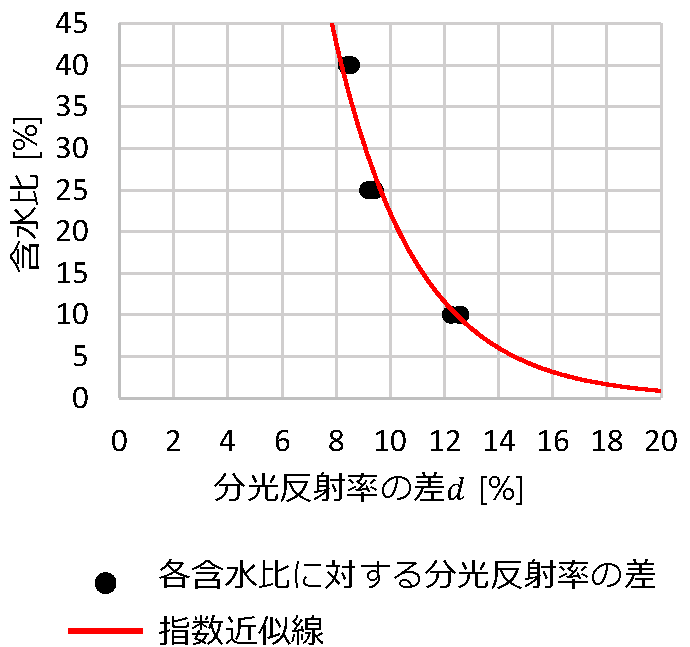
\includegraphics[width=8cm]{./Ch4_WaterContentEstimation/Fig/model_fitting_compressed.pdf}
	\caption{含水比と分光反射率の差の関係への指数近似線のフィッティング}\label{fig:model_fitting}
	\vspace{0.5cm}
	\end{center}
\end{figure}

\clearpage


%==============================================================================
%含水比を推定する検証実験
%==============================================================================
\section{含水比を推定する検証実験}
\label{sec:PreliminaryExperimentOfEstimation}

\ref{sec:EstimationFromSpectrum}節と\ref{sec:AnalysisOfMultispectralImage}節で解説した,
マルチスペクトル画像から取得した水が光を吸収する近赤外の波長帯と水が光を吸収しない波長帯の2つの波長帯の分光反射率の差を用いた,
含水比推定の手法の有効性を確認するため,
検証実験を行った.

\subsection{実験環境}
\label{ssec:EstimationExperimentSetting}

今回の検証実験の目的は,水による光の吸収度合いが異なる2つの波長帯の分光反射率の差を用いて,含水比を推定できるか確認することである.
そこで,同じ種類の土に対して含水比が10\%,25\%,40\%の合計3つのサンプルを用意し,
そして,屋外でそのサンプルのマルチスペクトル画像を撮影した.
マルチスペクトル画像を撮影した様子を図\ref{fig:watercontent_estimation_experiment_setting}に示す.
図\ref{fig:watercontent_estimation_experiment_setting}に示す通り,同じ種類だが異なる含水比の土のサンプル3つと,分光反射率スペクトルが分かっている校正用シートを
並べて撮影した.
サンプルと校正用シートの並び順を図\ref{fig:watercontent_estimation_experiment_sample_arrangement}に示す.
% そして,マルチスペクトル画像を撮影するためのマルチスペクトルカメラを土を入れた容器の直情に配置して,撮影を行った.
また,今回の検証実験で使用したマルチスペクトルカメラは,TETRACAM製のMacawである.
Macawの写真を図\ref{fig:multispectral_camera}に示す.
また,Macawの具体的な仕様を表\ref{tbl:multispectral_camera}に示す.

\begin{figure}[p]
	\begin{center}
		\begin{tabular}{c}

			\begin{minipage}[t]{\linewidth}
			\hspace{3cm}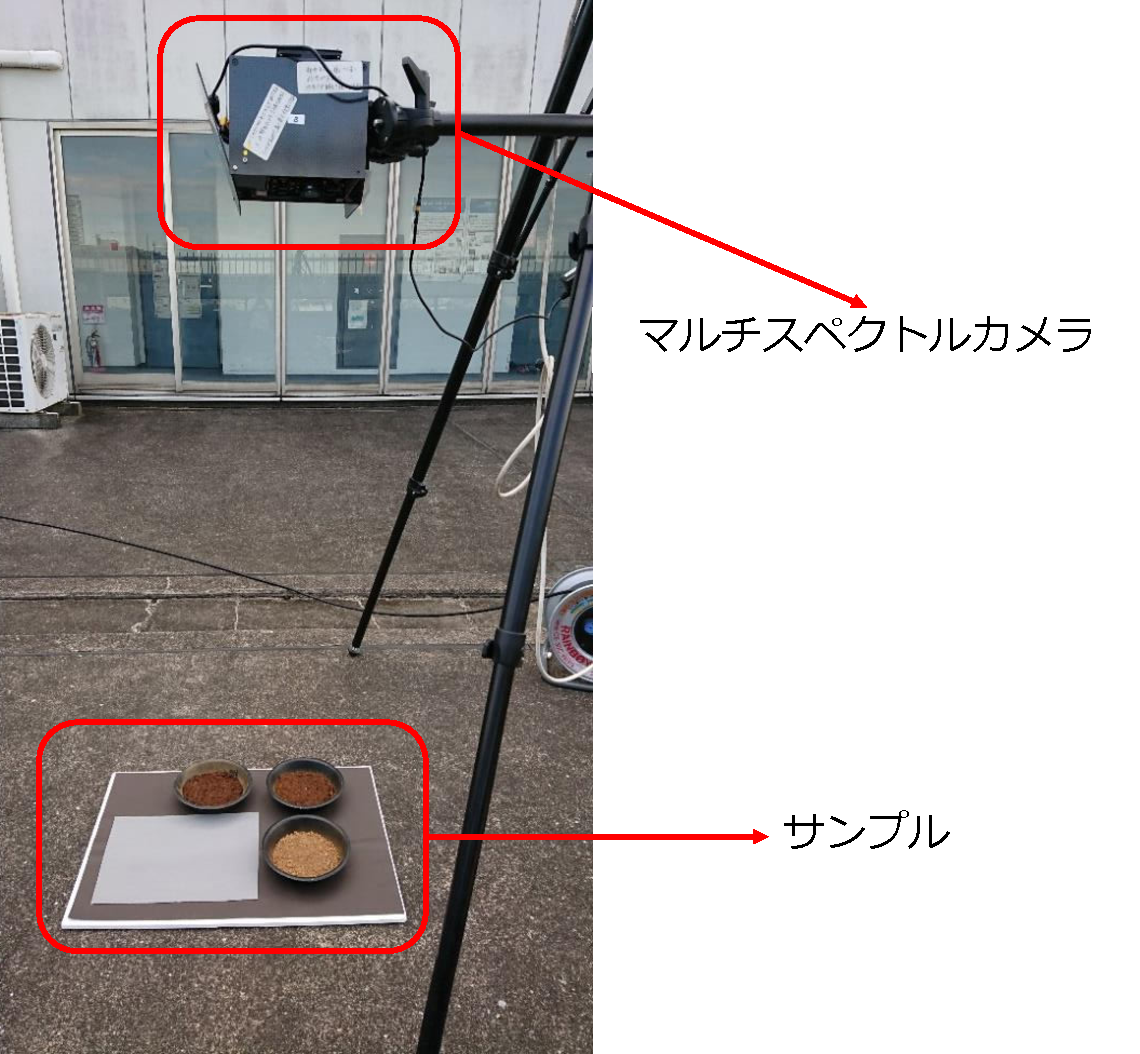
\includegraphics[width=9cm]{./Ch4_WaterContentEstimation/Fig/watercontent_estimation_experiment_setting_compressed.pdf}
			\caption{含水比推定の検証実験における撮影機材の配置}\label{fig:watercontent_estimation_experiment_setting}
			\vspace{2cm}
			\end{minipage}

			\\

			\begin{minipage}[b]{\linewidth}
			\centering
			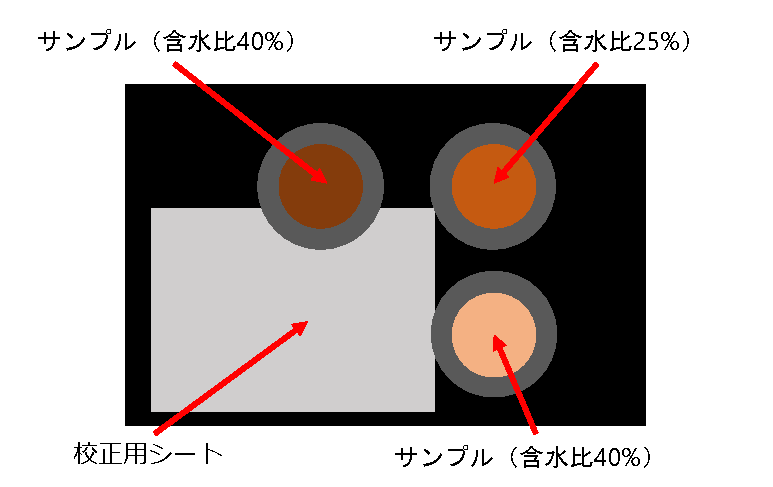
\includegraphics[width=12cm]{./Ch4_WaterContentEstimation/Fig/watercontent_estimation_experiment_sample_arrangement_compressed.pdf}
			\caption{含水比推定の検証実験における異なる含水比のサンプルの配置}\label{fig:watercontent_estimation_experiment_sample_arrangement}
			\end{minipage}

		\end{tabular}
	\end{center}
\end{figure}


\begin{figure}[p]
	\begin{center}
		\begin{tabular}{c}

			\begin{minipage}[t]{\linewidth}
			\hspace{4cm}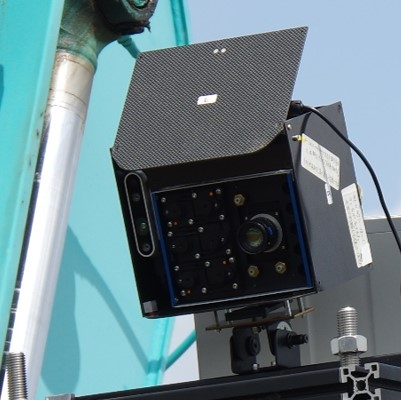
\includegraphics[width=6cm]{./Ch4_WaterContentEstimation/Fig/multispectral_camera.jpg}
			\caption{Macaw}\label{fig:multispectral_camera}
			\vspace{2cm}
			\end{minipage}

			\\

			\begin{minipage}[b]{\linewidth}

			\tblcaption{Macawの仕様}\label{tbl:multispectral_camera}

				\hspace{4cm} \begin{tabular}{|c|c|} \hline % 表の位置が左に寄りすぎないように調整
				製品名 & Macaw \\
				(メーカー) & (TETRACAM) \\ \hline
				波長 & 490nm, 570nm, 671nm \\ 
				     & 800nm, 900nm, 950nm \\
				     & 900 $\sim$ 1700nm \\ \hline
				波長帯数 & 7 \\ \hline
				\end{tabular}
			\end{minipage}

		\end{tabular}
	\end{center}
\end{figure}
 
\clearpage

\subsection{実験データ}
\label{ssec:EstimationExperimentalProcedure}

今回の実証実験では,\ref{sec:PreliminaryExperimentOfDiscrimination}節で解説した土の種類を識別する検証実験で使用した10種類の土のうち,
粘性土と火山灰質粘性土によって構成される5種類の細粒土を使用した.% この5種類の細粒度は,粘性土と呼ばれる土に属している.
砂質土や礫質土が,含水比の増減に関係なく建設機械の走破が可能な程度のコーン指数を維持するのに対し,
火山灰質粘性土も含む粘性土は,含水比が上昇すると建設機械の走破が困難になるほどコーン指数を低下させる土であることが知られている\cite{Meyer1961}.% "コーン指数"には低下という言葉を使用する
そこで,この検証実験においても,5種類の粘性土を対象として含水比推定の検証実験を行った.
今回使用する粘性土は,\ref{sec:PreliminaryExperimentOfDiscrimination}節で使用した10種類の土のうちの,
A, B, D, F, Gの粘性土である.
この5種類の粘性土のRGB画像を図\ref{fig:watercontent_estimation_experiment_data}に示す.

% \begin{figure}[p]
% 	\begin{center}
% 	\centering
% 	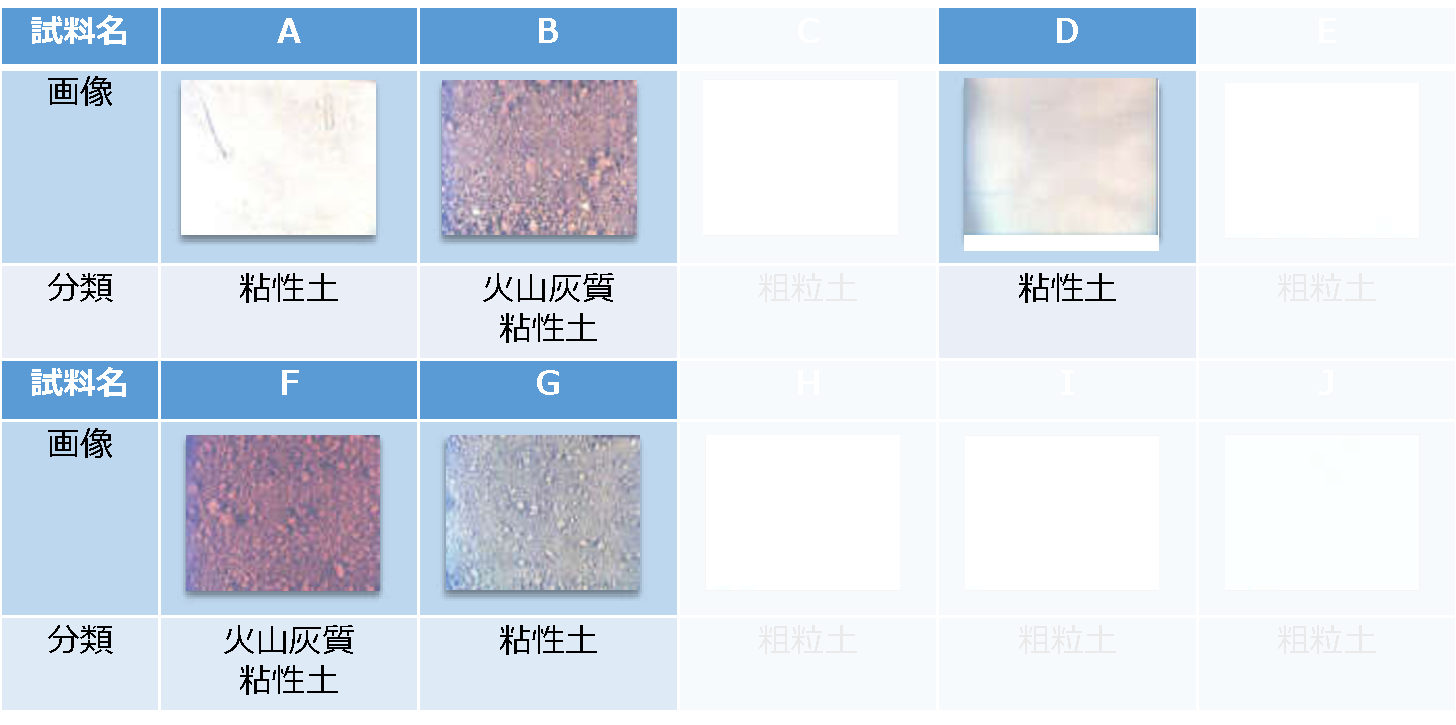
\includegraphics[width=15cm]{./Ch4_WaterContentEstimation/Fig/watercontent_estimation_experiment_data_compressed.pdf}
% 	\caption{含水比推定の検証実験用のデータ}\label{fig:watercontent_estimation_experiment_data}
% 	\end{center}
% \end{figure}

\begin{figure}[b]
	\begin{center}
		\begin{tabular}{c}

			\begin{minipage}[t]{0.33\linewidth}
			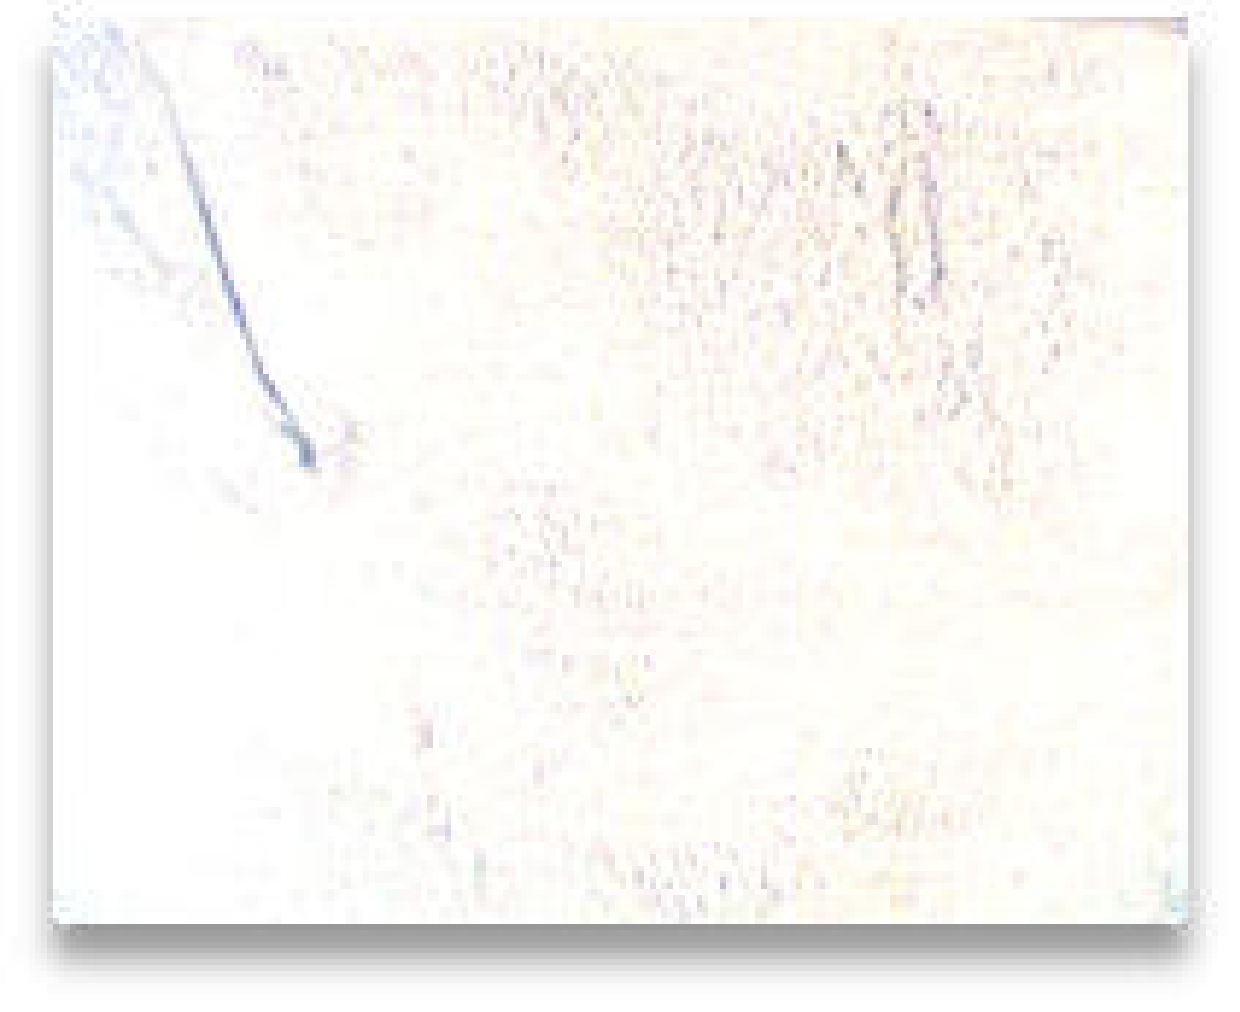
\includegraphics[width=4cm]{./Ch3_SoilTypeDiscrimination/Fig/A_Fu_image_compressed.pdf}
			\caption*{(a)土の種類A(粘性土)}%\label{fig:spectrum_for_different_soiltype}
			% \vspace{2cm}
			\end{minipage}

			\begin{minipage}[t]{0.33\linewidth}
			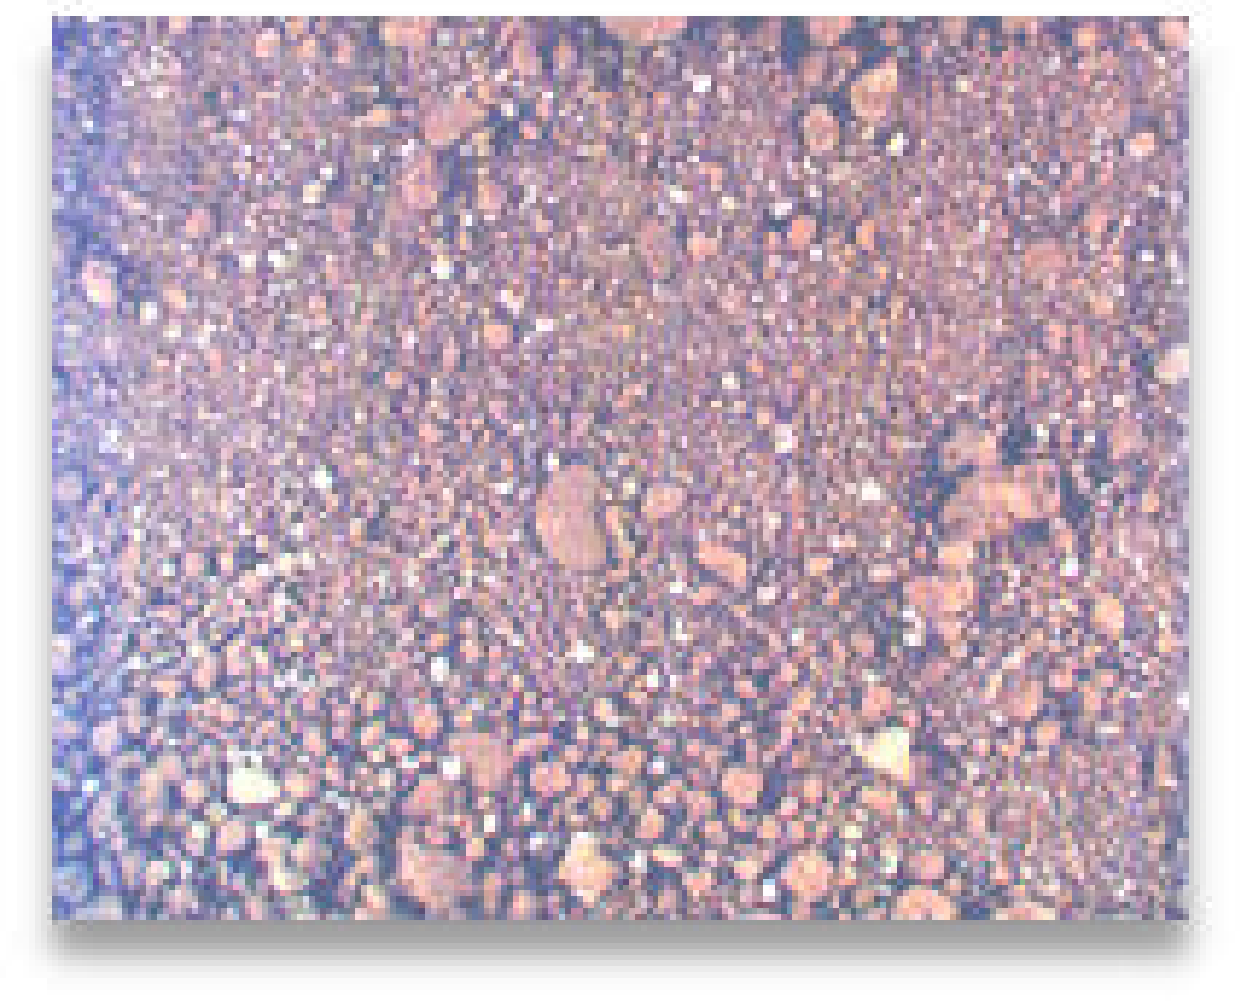
\includegraphics[width=4cm]{./Ch3_SoilTypeDiscrimination/Fig/B_Is_image_compressed.pdf}
			\caption*{(b)土の種類B(火山灰質粘性土)}
			\end{minipage}

			\hfill

			% \begin{minipage}[t]{0.33\linewidth}
			% 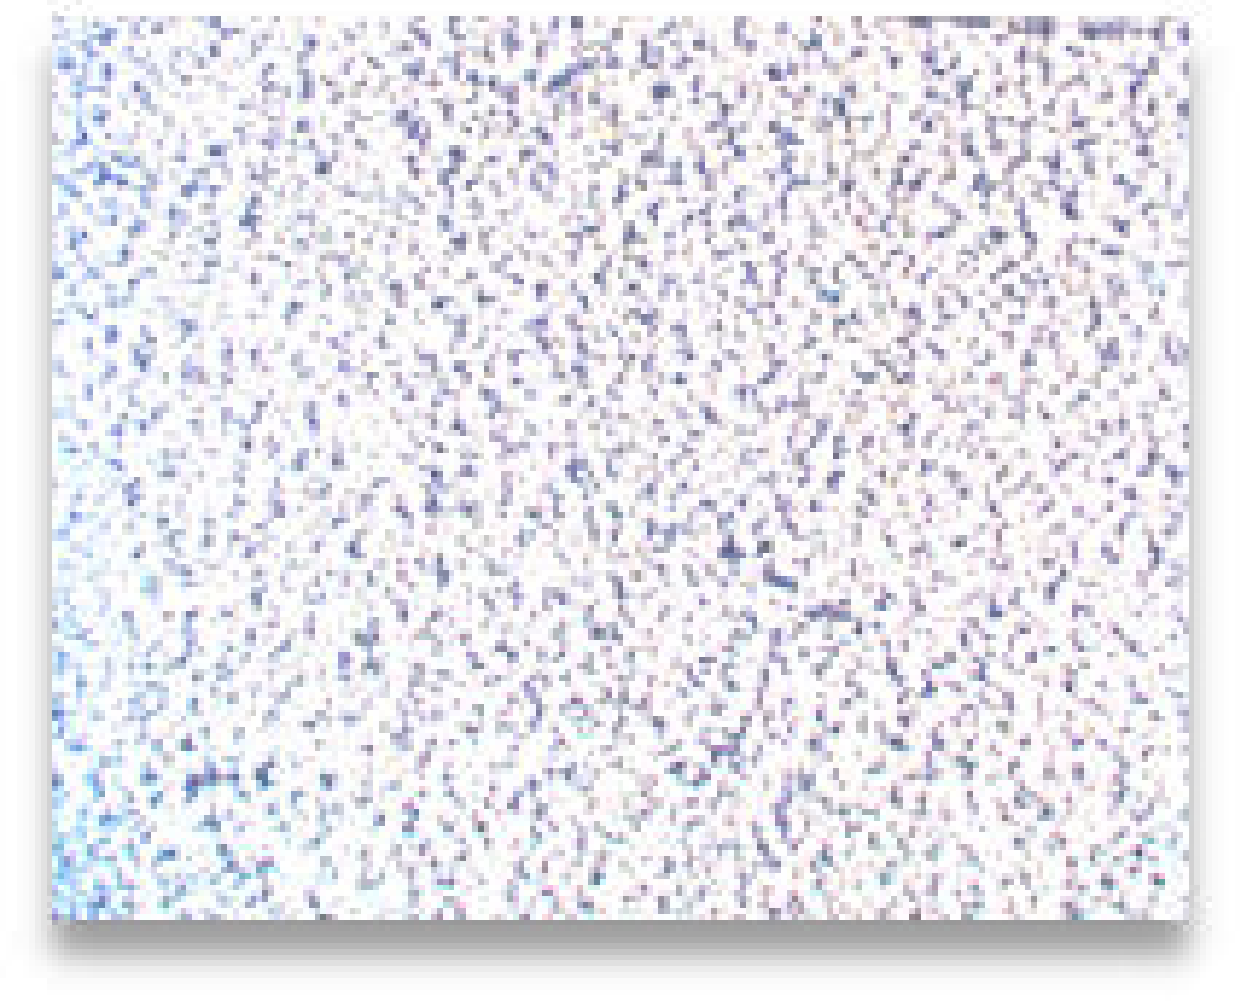
\includegraphics[width=4cm]{./Ch3_SoilTypeDiscrimination/Fig/C_K1_image_compressed.pdf}
			% \caption*{土の種類C(粗粒土の1種)}
			% \end{minipage}

			

			\begin{minipage}[t]{0.33\linewidth}
			
\includegraphics[width=4cm]{./Ch3_SoilTypeDiscrimination/Fig/D_K9_image_compressed.pdf}
			\caption*{(c)土の種類D(粘性土)}%\label{fig:spectrum_for_different_soiltype}
			% \vspace{2cm}
			\end{minipage}

			\\

			% \begin{minipage}[t]{0.33\linewidth}
			% 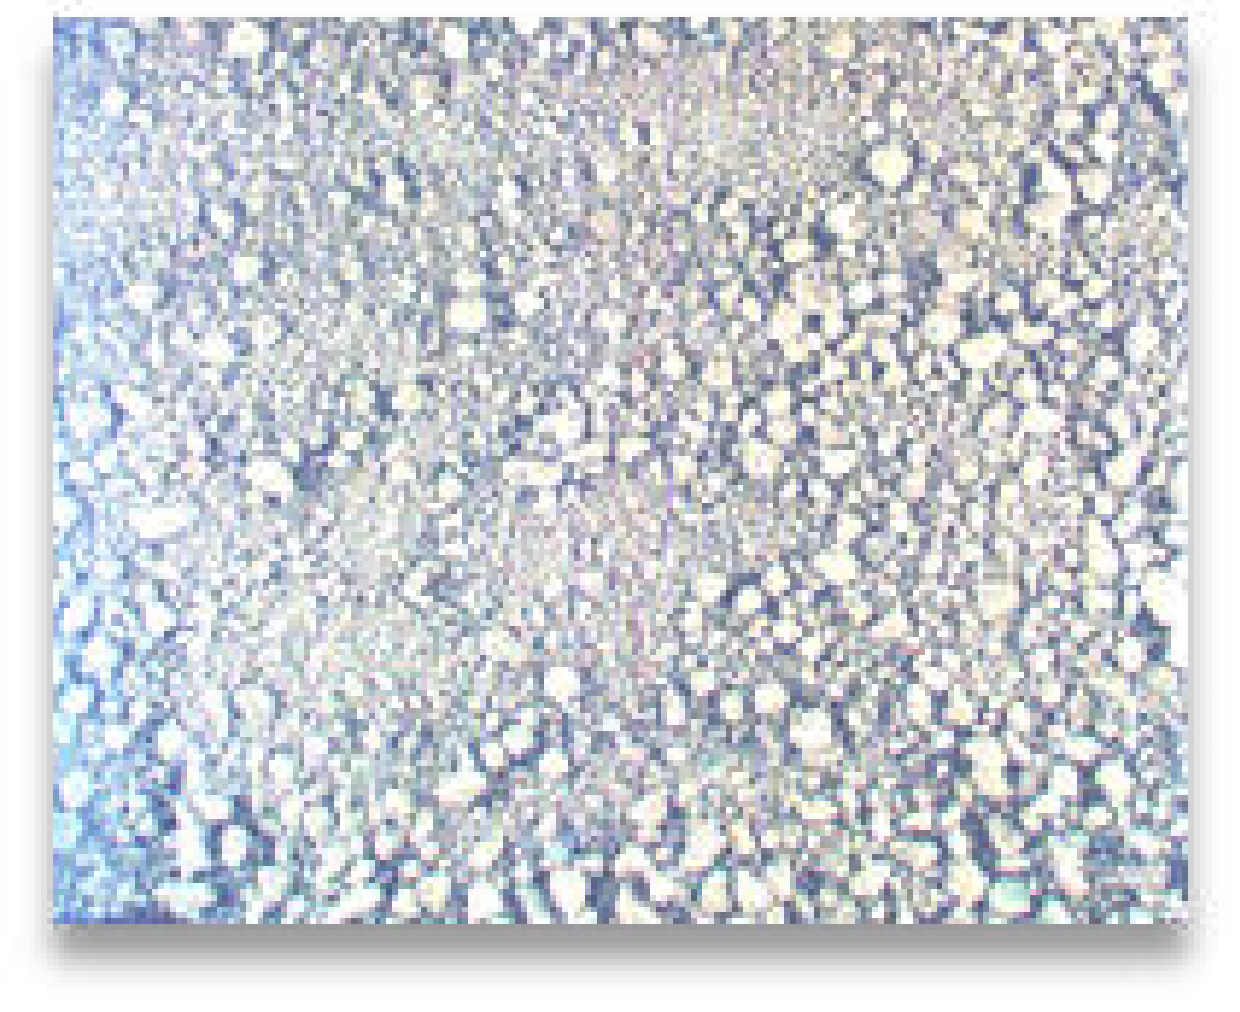
\includegraphics[width=4cm]{./Ch3_SoilTypeDiscrimination/Fig/E_Ko_image_compressed.pdf}
			% \caption*{土の種類E(粗粒土の1種)}
			% \end{minipage}

			% \hfill

			\begin{minipage}[t]{0.33\linewidth}
			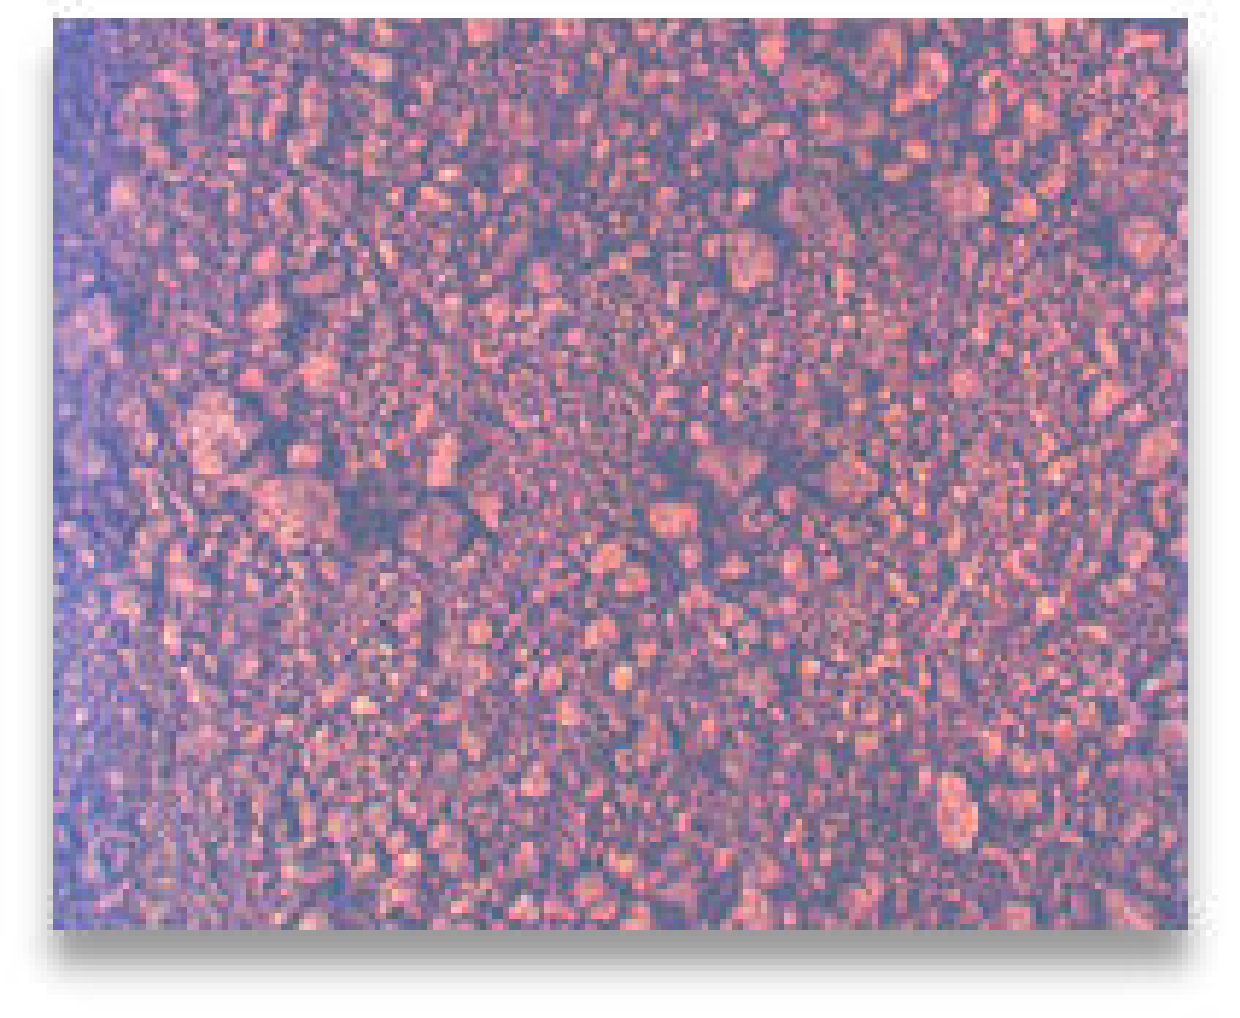
\includegraphics[width=4cm]{./Ch3_SoilTypeDiscrimination/Fig/F_Lo_image_compressed.pdf}
			\caption*{(d)土の種類F(火山灰質粘性土)}
			\end{minipage}

			% \\

			\begin{minipage}[t]{0.33\linewidth}
			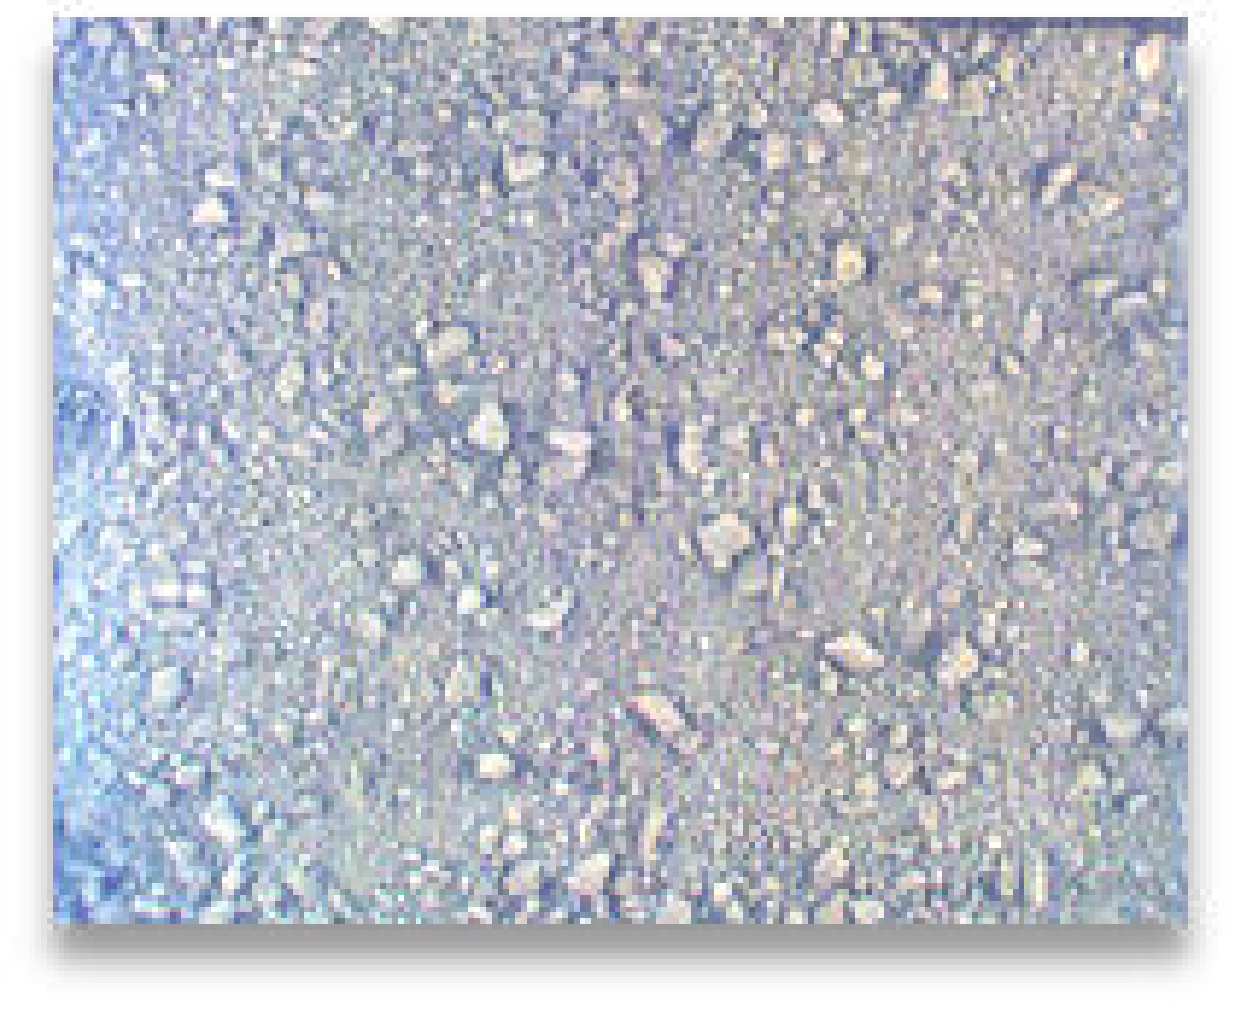
\includegraphics[width=4cm]{./Ch3_SoilTypeDiscrimination/Fig/G_Mi_image_compressed.pdf}
			\caption*{(e)土の種類G(粘性土)}%\label{fig:spectrum_for_different_soiltype}
			% \vspace{2cm}
			\end{minipage}

			% \begin{minipage}[t]{0.33\linewidth}
			% 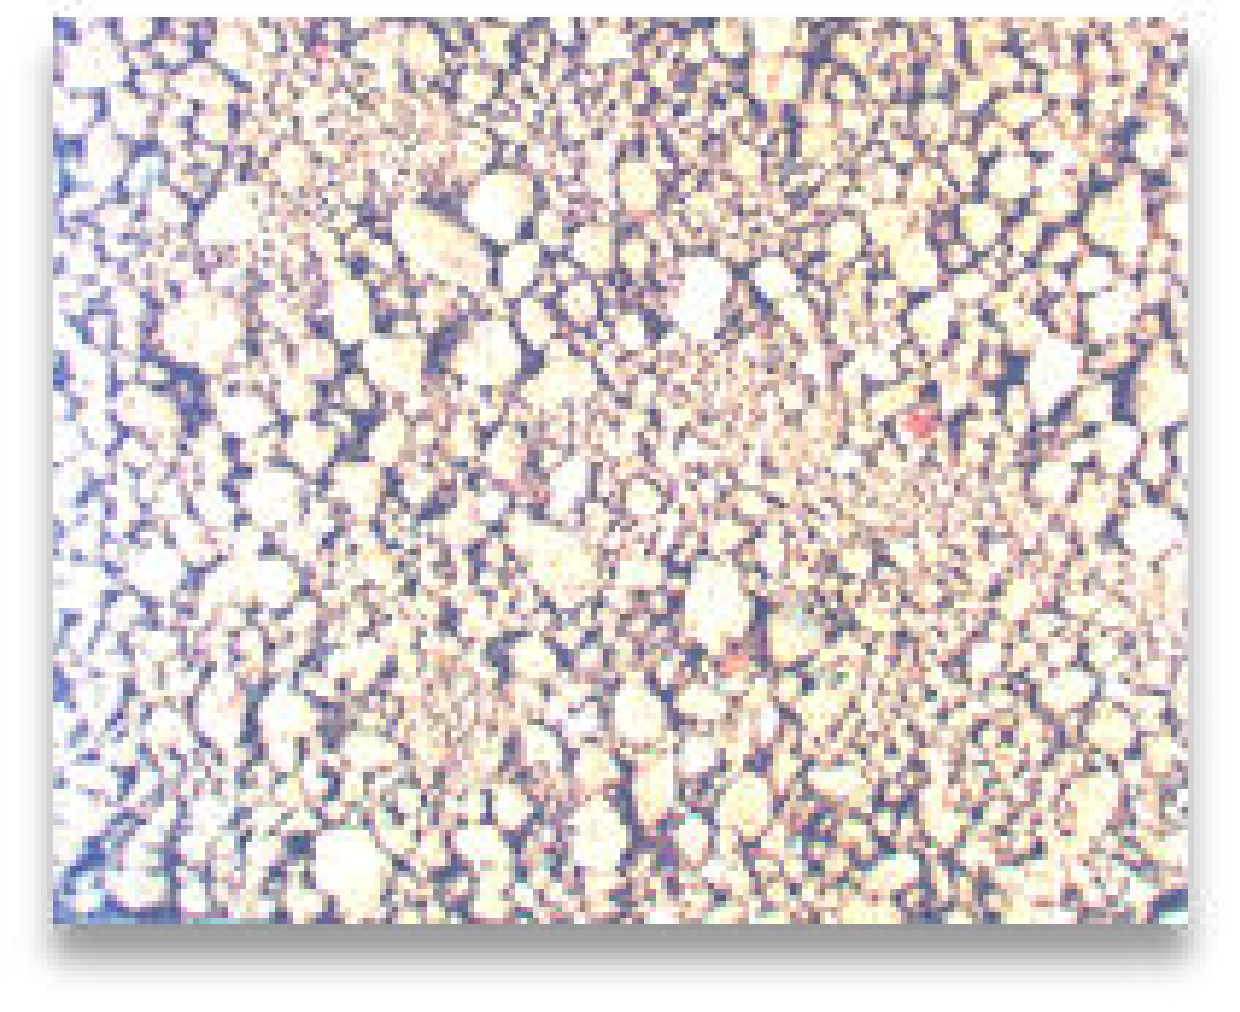
\includegraphics[width=4cm]{./Ch3_SoilTypeDiscrimination/Fig/H_Oh_image_compressed.pdf}
			% \caption*{土の種類H(粗粒土の1種)}
			% \end{minipage}

			% \hfill

			% \begin{minipage}[t]{0.33\linewidth}
			% 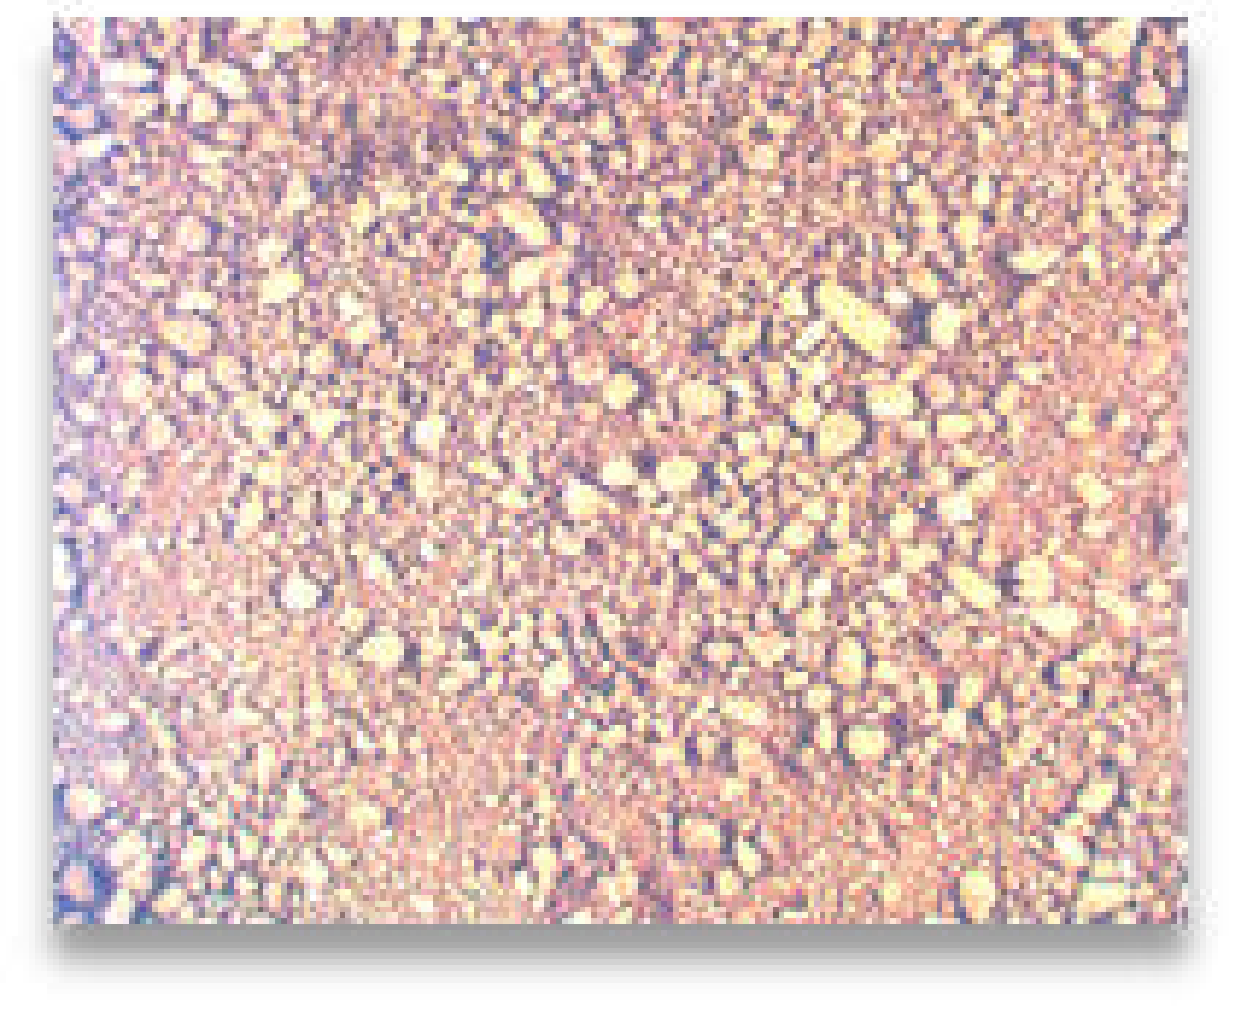
\includegraphics[width=4cm]{./Ch3_SoilTypeDiscrimination/Fig/I_Sa_image_compressed.pdf}
			% \caption*{土の種類I(粗粒土の1種)}
			% \end{minipage}

			% \\

			% \begin{minipage}[t]{0.33\linewidth}
			% 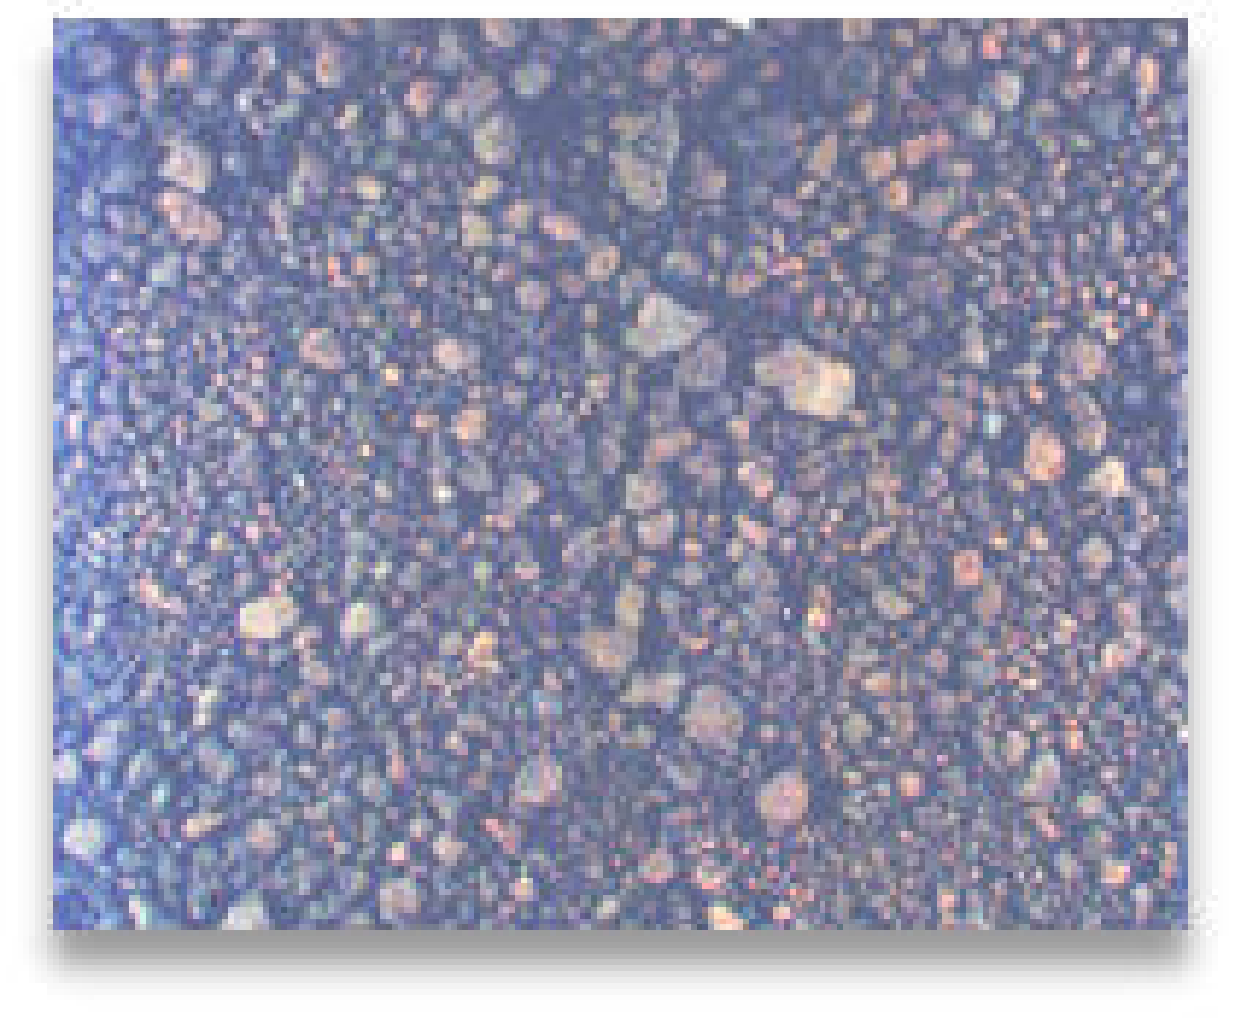
\includegraphics[width=4cm]{./Ch3_SoilTypeDiscrimination/Fig/J_Sc_image_compressed.pdf}
			% \caption*{土の種類J(粗粒土の1種)}
			% \end{minipage}

		\end{tabular}
		\caption{含水比推定の検証実験用のデータ}\label{fig:watercontent_estimation_experiment_data}
	\end{center}
\end{figure}

\clearpage


\subsection{実験結果}
\label{ssec:EstimationResult}

\ref{sec:AnalysisOfMultispectralImage}節で解説した手法を用いて,
900 $\sim$ 1700nmの波長帯と570nmの波長帯の分光反射率の差に指数近似線をフィッティングさせた様子を
図\ref{fig:watercontent_estimation_fitting}に示す.
図\ref{fig:watercontent_estimation_fitting}にある各グラフは,\ref{ssec:AnalysisOfSpectrum}節で示した図\ref{fig:model_fitting}のグラフと同様に,
縦軸は含水比を示しており,横軸は2つの波長帯の分光反射率の差を示している.
また,各グラフにおいて,黒い点が撮影したマルチスペクトル画像から取得した900 $\sim$ 1700nmの波長帯と570nmの波長帯の分光反射率の差と
含水比の関係をプロットした点であり,赤い曲線がそのプロットされた黒い点にフィッティングされた指数近似線を示す.
図\ref{fig:watercontent_estimation_fitting}にある各グラフおよびそのグラフに示された決定係数$R^2$から分かる通り,今回の含水比推定の検証実験で使用した5種類の粘性土において,モデルフィッティングが成功したことが分かる.
% 各グラフに示された決定係数$R^2$からもそれが分かる.

\begin{figure}[p]
	\begin{center}
		\begin{tabular}{c} % 隣り合う図がずれないようにする

			\hspace{-1cm}\begin{minipage}[b]{0.5\linewidth}
			\centering
			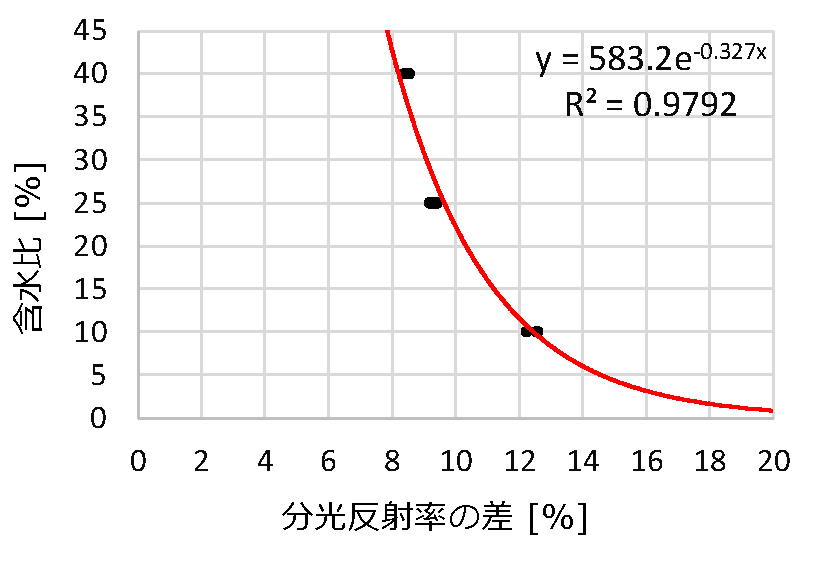
\includegraphics[width=7cm]{./Ch4_WaterContentEstimation/Fig/image_Fu(A)watercontent_spectrum_relationship_compressed.pdf}
			\caption*{(a)土の種類A}
			\end{minipage}

			\hfill

			\begin{minipage}[b]{0.5\linewidth}
			\centering
			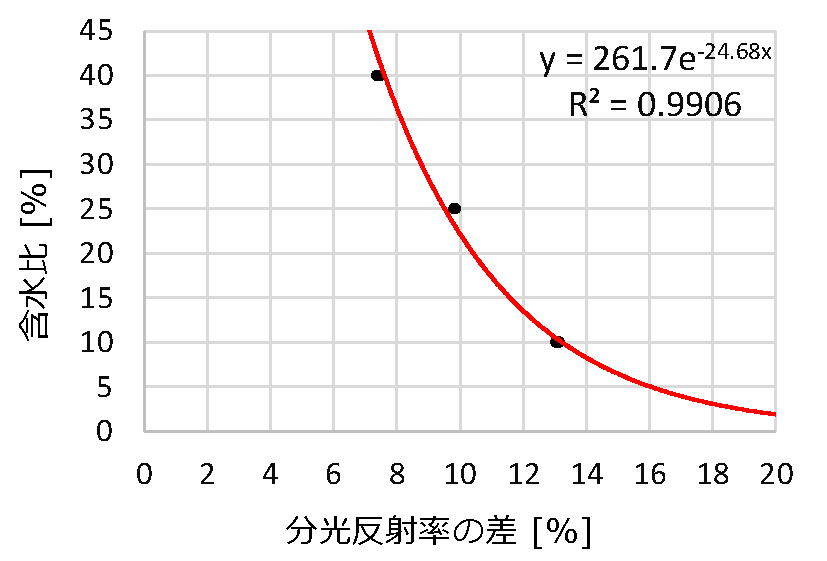
\includegraphics[width=7cm]{./Ch4_WaterContentEstimation/Fig/image_Is(B)watercontent_spectrum_relationship_compressed.pdf}
			\caption*{(b)土の種類B}
			\end{minipage}

			\\

			\hspace{-1cm}\begin{minipage}[b]{0.5\linewidth}
			\centering
			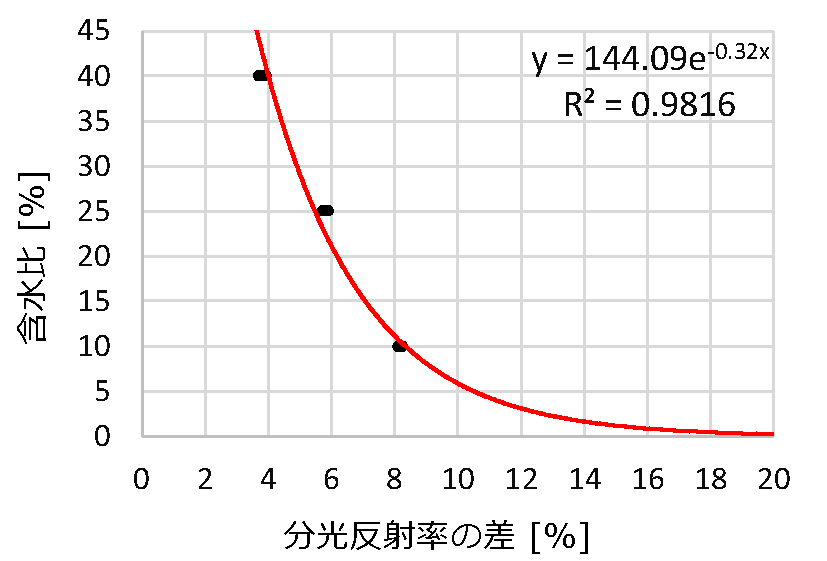
\includegraphics[width=7cm]{./Ch4_WaterContentEstimation/Fig/image_K9(D)watercontent_spectrum_relationship_compressed.pdf}
			\caption*{(c)土の種類D}
			\end{minipage}

			\hfill

			\begin{minipage}[b]{0.5\linewidth}
			\centering
			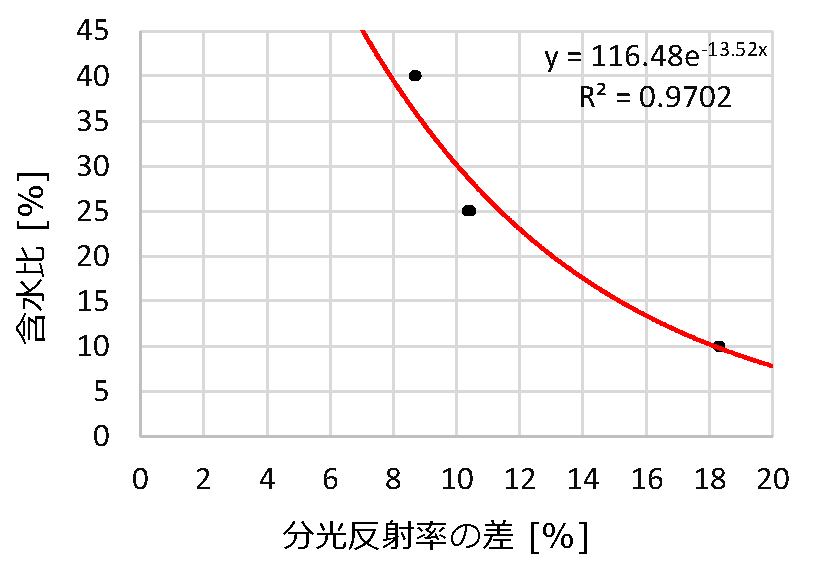
\includegraphics[width=7cm]{./Ch4_WaterContentEstimation/Fig/image_Lo(F)watercontent_spectrum_relationship_compressed.pdf}
			\caption*{(d)土の種類F}
			\end{minipage}

			\\

			\hspace{-1cm}\begin{minipage}[b]{0.5\linewidth}
			\centering
			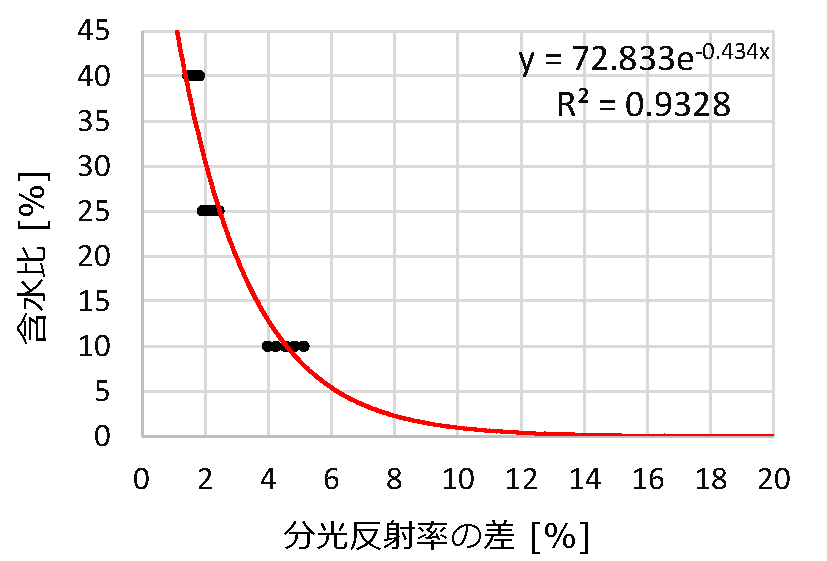
\includegraphics[width=7cm]{./Ch4_WaterContentEstimation/Fig/image_Mi(G)watercontent_spectrum_relationship_compressed.pdf}
			\caption*{(e)土の種類G}
			\end{minipage}

			\hfill

			\begin{minipage}[b]{0.5\linewidth}
			\centering
			\vspace{-3cm}
			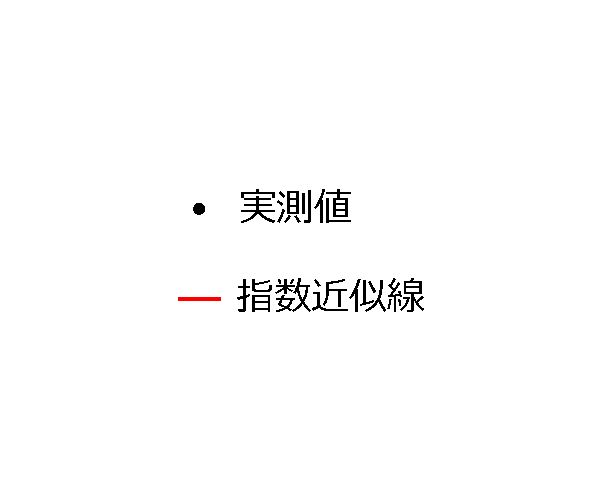
\includegraphics[width=5cm]{./Ch4_WaterContentEstimation/Fig/legend_of_watercontent_spectrum_relationship_compressed.pdf}
			\end{minipage}

		\end{tabular}
	\caption{含水比推定のための指数近似線によるフィッティング}\label{fig:watercontent_estimation_fitting}
	\end{center}
\end{figure}

\clearpage


\subsection{考察}
\label{ssec:EstimationConsideration}

\ref{ssec:EstimationResult}項で示した含水比推定の検証実験の結果より,
マルチスペクトル画像から取得した,水が光を吸収する近赤外の波長帯と,水が光を吸収しない波長帯の分光反射率の,2つの分光反射率の差を用いた
含水比の推定が可能であることが分かった.
水が近赤外の光を吸収することを利用した含水比の推定手法が上手くいった原因は,
マルチスペクトル画像を用いて近赤外の広い範囲の光を1つの波長帯として分光させたため,
温度や湿度の変動による近赤外の光を吸収する波長帯の多少の変動には頑強であったためである.

しかし,図\ref{fig:watercontent_estimation_fitting}(d)のFの土のグラフに示した,含水比が40$\%$や25$\%$のプロットのように,
水が光を吸収する近赤外の波長帯と水が光を吸収しない波長帯の分光反射率の差と含水比の関係をプロットした点の一部は,
近似線から離れたところにあることも分かった.
これは,\ref{ssec:RelationshipBetweenSpectrumAndWaterContent}項で述べたように,
含水比の増加に伴い,
空気と土の間の屈折率の差が減少するため,
空気中から土への入射光の内,反射せずに土の中に屈折して進入していく光の割合が増えるため,
水が光を吸収しない波長帯の分光反射率も含水比の増加に伴い変動するためである.
水が光を吸収しない波長帯の分光反射率が大きく変動すると,
水が光を吸収する近赤外の波長帯と光を吸収しない波長帯の差に影響を与え,
分光反射率の差を用いた含水比の推定の難易度が上昇する.
この変動を抑制するためには,
近赤外線以外の,水が光を吸収しない波長帯に,
本論文の中で使用した570nmの波長帯よりも,含水比の増加に伴う分光反射率の変動の少ない波長帯を探索する必要がある.

\newpage

%==============================================================================
%おわりに
%==============================================================================
\section{おわりに}

本章では,本研究で提案した非接触での走破性判定のための手法の2つ目のステップである,
スペクトル画像を用いた含水比の推定の詳細について述べた.

まず,\ref{sec:EstimationFromSpectrum}節において,
水分子がその構成原子である酸素原子と水素原子の間の振動収縮と変角運動によって
近赤外の光を吸収することを利用し,水が光を吸収する近赤外の波長帯と水が光を吸収しない波長帯の分光反射率の差を用いて
含水比を推定することを述べた.

次に,\ref{sec:AnalysisOfMultispectralImage}節において,
マルチスペクトル画像から取得した分光反射率の差を用いて含水比を推定する手法の詳細を述べた.
本研究では,含水比と水が光を吸収する近赤外の波長帯と水が光を吸収しない波長帯の分光反射率の差の関係に対して,
指数近似線をフィッティングさせることによって含水比を推定した.
% ,その指数近似線を用いて新たなマルチスペクトル画像から取得した
% 2つの波長帯の分光反射率の差によって含水比を推定する.

最後に,\ref{sec:PreliminaryExperimentOfEstimation}節において,
\ref{sec:EstimationFromSpectrum}節と\ref{sec:AnalysisOfMultispectralImage}節で解説した,
マルチスペクトル画像から含水比を推定する手法の有効性を確認するために,含水比推定の検証実験を行った.
検証実験の結果,含水比と分光反射率の差の関係に対して近似線がフィッティングしたため,
マルチスペクトル画像から含水比を推定することが可能であることが分かった.

\newpage
%%%%%%%%%%%%%%%%%%%%%%%%%%%%%%%%%%%%%%%%%%%%%%%%%%%%%%%%%%%%%%%%%%%%%%%%%%%%%%%